% Native PGFPlots; generated by examples/generate_figures.py.
% Constructed or analytical teaching example.
\begingroup
\definecolor{blueplot}{HTML}{4E79A7}
\definecolor{redplot}{HTML}{D95F59}
\definecolor{inkplot}{HTML}{111111}
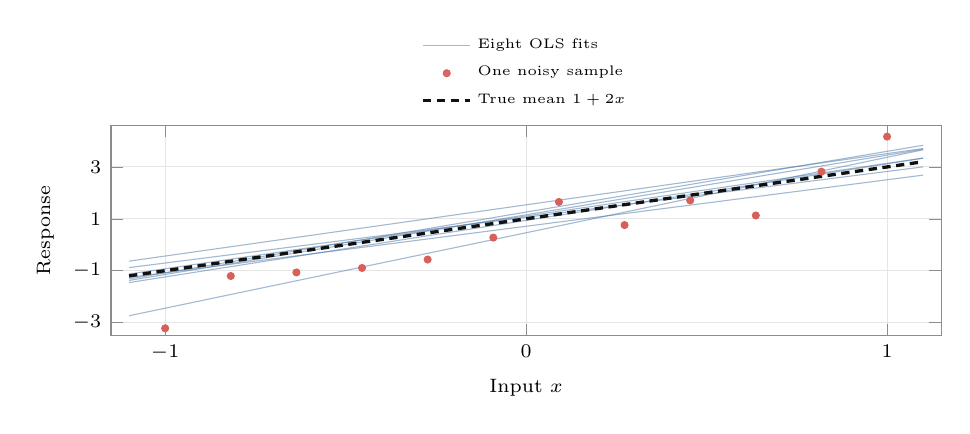
\begin{tikzpicture}
\begin{axis}[
width=\linewidth,height=4.25cm,font=\scriptsize,
tick label style={font=\scriptsize},label style={font=\scriptsize},
axis line style={black!45},tick style={black!45},
grid=major,grid style={black!10},scaled ticks=false,
clip=true,unbounded coords=jump,
legend style={font=\tiny,draw=none,fill=white,fill opacity=.94,text opacity=1,
  legend cell align=left,inner sep=2pt,row sep=1pt},
xmin=-1.15,xmax=1.15,ymin=-3.5,ymax=4.6,
xlabel={Input $x$},ylabel={Response},xtick={-1,0,1},ytick={-3,-1,1,3},
legend style={at={(.5,1.03)},anchor=south}
]
\addplot[blueplot,opacity=.52,thin,no marks] coordinates {(-1.1,-2.736812662) (1.1,3.66131734)};
\addlegendentry{Eight OLS fits}
\addplot[blueplot,opacity=.52,thin,no marks,forget plot] coordinates {(-1.1,-0.6330407098) (1.1,3.71140742)};

\addplot[blueplot,opacity=.52,thin,no marks,forget plot] coordinates {(-1.1,-1.259051388) (1.1,2.683528342)};

\addplot[blueplot,opacity=.52,thin,no marks,forget plot] coordinates {(-1.1,-1.376008947) (1.1,3.683388137)};

\addplot[blueplot,opacity=.52,thin,no marks,forget plot] coordinates {(-1.1,-1.128457041) (1.1,3.340279621)};

\addplot[blueplot,opacity=.52,thin,no marks,forget plot] coordinates {(-1.1,-1.317027287) (1.1,3.835395999)};

\addplot[blueplot,opacity=.52,thin,no marks,forget plot] coordinates {(-1.1,-1.458337047) (1.1,3.338370423)};

\addplot[blueplot,opacity=.52,thin,no marks,forget plot] coordinates {(-1.1,-0.8811701508) (1.1,3.001774785)};

\addplot[only marks,mark=*,mark size=1.25pt,redplot] coordinates {(-1,-3.22111805) (-0.8181818182,-1.205099716) (-0.6363636364,-1.067589845) (-0.4545454545,-0.8944359831) (-0.2727272727,-0.5705664) (-0.09090909091,0.2752890744) (0.09090909091,1.650128788) (0.2727272727,0.7592475727) (0.4545454545,1.707761163) (0.6363636364,1.128217599) (0.8181818182,2.816360351) (1,4.168833518)};
\addlegendentry{One noisy sample}
\addplot[inkplot,very thick,densely dashed,no marks,domain=-1.1:1.1] {1+2*x};
\addlegendentry{True mean $1+2x$}
\end{axis}
\end{tikzpicture}
\endgroup
